\documentclass[]{llncs}
\usepackage[utf8]{inputenc}
\usepackage[hidelinks]{hyperref}
\usepackage[numbers,sort,compress]{natbib}
\usepackage{graphicx}

\begin{document}

\title{Assessment of Transcription Factor Binding Motif and Regulon Transfer
  Methods}
\author{Sefa Kilic \and Ivan Erill}
\institute{University of Maryland Baltimore County\\
Department of Biological Sciences\\
1000 Hilltop Circle, Baltimore, Maryland 21250\\
\email{\{sefa1,erill\}@umbc.edu}}

\maketitle

\begin{abstract}
  Despite its fundamental importance in comparative genomics studies, the impact
  of motif transfer methods remains largely unstudied. With the recent increase
  in availability of transcription factor binding site data from traditional and
  high-throughput experiments, it has become possible to assess existing
  comparative genomics approaches as well as to benchmark newly developed
  ones. In this study, we describe three different transfer methods that define
  transcription factor binding motif in a target species given some regulatory
  activity information in a reference species. We evaluate these methods and
  report their performances on identifying binding sites, binding motif and
  regulon for a given genome.
\end{abstract}

\section{Introduction}
Comparative genomics has been leveraged in many studies to characterize
transcriptional regulatory networks~\cite{gelfand2000prediction,
  ravcheev2013genomic, meireles2009comparative,kellis2004methods}. By analyzing
the degree of conservation of functional elements across multiple genomes,
comparative genomics analyses make it possible to reconstruct regulatory
networks in multiple species. Thanks in large part to high-throughput
experimental techniques (e.g., ChIP-seq~\cite{bailey2013practical}), available
experimental binding site data has increased dramatically over the last few
years and it has become possible for the first time to reliably assess methods
used for regulatory network reconstruction.

Given a transcription factor (TF) and some reference information on its
regulatory activity, the main steps of transcriptional regulatory network
reconstruction are (a) transferring the available information (i.e., known
binding sites and regulated genes for a TF) from reference species to define
binding motif in target species, (b) searching target species with transferred
motif to estimate its regulatory network (or regulon) and (c) filtering false
positives via comparative analysis of putative target sites. In the transfer
step, the goal is to define a putative motif based on a reference one. This
motif is then used to search the genome for putative sites. The final step,
called “consistency check”~\cite{rodionov2007comparative}, is based on the idea
that true sites are likely to be present upstream of orthologous regulated
genes, while false positives should be scattered randomly and not consistently
across genomes~\cite{tan2001comparative, mironov1999computer,
  makarova2001conservation, rodionov2000transcriptional, panina2001comparative,
  leyn2011control, rodionov2004reconstruction, kazakov2009comparative}.

In this study, we focus on the first step of the comparative genomics pipeline:
the transfer method. To evaluate different methods we define the goal as the
ability to identify binding sites, binding motif and regulon for a TF in a
genome, given the collection of experimentally validated binding sites for the
same TF in a reference genome. This can be achieved using the known motif or
network structure as prior information. Motif-based transfer is performed using
the reference binding motif to search for putative binding sites in the target
genome. The underlying assumption is that, for a given TF, the binding motif is
relatively well conserved across closely related species. This method has been
shown to perform well at inferring existing regulatory networks in previously
uncharacterized genomes~\cite{mironov1999computer, tan2001comparative,
  rodionov2008transcriptional, erill2004differences}. The other source of prior
information that can be used is the regulatory network itself. The putative
regulon is then constructed based on orthologous transfer of the reference
regulon and \textit{de novo} motif discovery is performed on the promoter
regions of putatively regulated target genes~\cite{shelton1997phylogenetic,
  panina2003comparative, mccue2001phylogenetic, wang2003combining,
  leyn2013genomic, zhang2009genome, zhang2010simultaneous}.

\section{Materials and Methods}
\subsection{Data}
Binding site data were compiled mainly from CollecTF, a database of
experimentally verified TFBS in Bacteria built by our group
\cite{kilic2013collectf}. As of October 2014, CollecTF had 4,942 experimentally
verified binding sites and associated gene regulation data for 229 TFs in 134
species, from 921 publications. Additional data were incorporated from
RegulonDB~\cite{salgado2013regulondb},
CoryneRegNet~\cite{pauling2012coryneregnet}, DBTBS~\cite{sierro2008dbtbs} and
MtbRegList~\cite{jacques2005mtbreglist}. The data from such databases were
downloaded and merged after removal of duplicates and of data without
experimental evidence. Table~\ref{tab:num_sites} shows the distribution of
binding sites in the compiled data by database.


\begin{table}{}
  \centering
  \caption{Number of experimentally validated binding sites by database}
  \begin{tabular}{lr}
    \hline\noalign{\smallskip}
    Database & Number of binding sites \\
    \noalign{\smallskip}
    \hline
    \noalign{\smallskip}
    CollecTF      &  4,942\\
    DBTBS         &  116\\
    MtbRegList    &  202\\
    CoryneRegNet  &  196\\
    RegulonDB     & 2,147\\
    \hline
    \end{tabular}
\label{tab:num_sites}
\end{table}

Complete genome sequences and annotations for species that have binding site
data were downloaded from NCBI RefSeq database. Operon predictions are based on
the DOOR database~\cite{mao2009door}. For binding site search, the regions
spanning from -300 bp to +50 bp relative to the corresponding gene translation
start site are used. Orthologs were detected using reciprocal
BLAST~\cite{wall2003detecting}.

\subsection{Direct Transfer}
The most straightforward motif transfer approach is the direct transfer using the
collection of known binding sites from a model
species~\cite{kazakov2009comparative, rodionov2011comparative}. Given a
collection of experimentally determined sites in the reference species, a
position-specific scoring matrix (PSSM)~\cite{stormo2000dna} is built and used
to scan the promoter regions of the genome of interest to identify putative
sites.

It is crucial to determine a threshold for PSSM search accurately. A low
threshold may classify most of the true binding sites correctly while producing
many false positives, whereas a high threshold is likely to miss many true
positives. One approach for threshold selection is to compute score distribution
of the PSSM and to specify a significance threshold~\cite{beckstette2006fast,
  staden1989methods,rahmann2003power}. Other commonly used approaches are to
define a threshold based on PSSM scores of known binding
sites~\cite{cornish2012inference, kazakov2013transcription} or to choose it
arbitrarily~\cite{kazakov2013transcription}. Another approach is to select a
fixed amount of highest scoring sites as putative binding
sites~\cite{lee2013lasagna}, essentially assuming that the size of the
regulatory network is conserved to a first approximation. For all motif transfer
methods in this study, the first $N_T$ highest scoring sites are selected as
putative sites, $N_T=\alpha{N_R}{G_T}/{G_R}$ where $N_R$ is the number of true
sites in the reference species, $G_T$ and $G_R$ are genome lengths for target
and reference species, respectively. $\alpha$ is used as a scaling factor, used
to increase sensitivity or specificity depending on the value of $\alpha$. It
should be noted that any bias introduced by this approach should be averaged out
as the transfer methods are tested both ways (i.e., using species A as reference
and B as target, and vice versa).

\subsection{PSSM Search Followed by Motif Discovery}
Another way of defining the binding motif in a target species is to perform
motif discovery on pre-searched candidate
sequences~\cite{habib2012functional}. First, the genome of interest is scanned
for putative target sites using the reference PSSM\@. A motif discovery
algorithm (e.g., MEME~\cite{bailey2006meme}) is then applied to the promoters of
high scoring sites. The motivation for this method is to capture motifs that are
slightly different from the reference one. It also mitigates the effect of an
inaccurate threshold for PSSM search. By choosing a relaxed threshold, this
method relies on well established motif discovery algorithms to identify a
conserved motif in the target species and disregards the regions with sites that
match the reference pattern but may not align well with the true target
motif. To prevent MEME from discovering motifs for other promoter elements, we
replace surrounding regions of putative sites with 100 bp sequences randomly
generated from genomic background, instead of using the promoters of
high-scoring sites directly for motif discovery.

\subsection{Network Transfer}
In closely related bacteria, it has been shown that orthologous TFs tend to have
conserved binding motifs~\cite{makarova2001conservation}. Although this tendency
has been observed among more distant bacteria for some TFs (e.g., ArgR/AhrC and
HrcA regulating arginine metabolism~\cite{maas1994arginine,
  klingel1995binding}), it does not hold for some other TFs such as the SOS
response repressor LexA in Gram-negative bacteria~\cite{wade2005genomic} and
DinR, its ortholog in Gram-positive bacteria~\cite{winterling1998bacillus}. An
important limitation of the motif-based transfer methods described above is that
they are expected to perform poorly if the motif is not conserved across
reference and target genomes. The underlying hypothesis for network transfer is
that the regulon across the reference and target genomes may be functionally
conserved to some degree even if the binding motif is not.

To define the motif in target species through network transfer, the first step
is to identify the set of operons that are regulated by the TF of interest. To
identify target regulon, genes that are orthologous to the ones in the reference
regulon are identified in the target species and their promoters, typically
shared with other genes in an operon configuration, are determined. In the next
step, these promoters are used for motif discovery. If genes of an operon in the
reference genome are dispersed into multiple operons in the target genome, all
promoters of such operons are included. The hypothesis is that this method makes
motif identification possible even if the motif is not conserved at all,
assuming the regulon is conserved to some extent.

\subsection{Performance Assessment}
To assess the performance of different transfer techniques quantitatively, we
measure both (a) the distance between the true motif and the inferred motif and
(b) the area under ROC curve for the inferred motif.  To measure the distance,
two motifs are aligned maximizing the alignment's information content. The
motif distance is then computed as the sum of Euclidean distances between
aligned columns of the two position specific frequency matrices
(PSFMs)~\cite{gupta2007quantifying, choi2004local}. ROC
curves~\cite{fawcett2006introduction, mathelier2013next,
  talebzadeh2014transcription, won2010genome, cornish2012inference} are computed
considering experimentally validated sites in target genomes as positives and
all other positions in promoter regions as negatives. To handle the problem of
class imbalance on binding site prediction, we selected same number of promoters
with and without true binding sites to compute ROC curves. To assess the
significance of performances for all three methods, we compute the distance and
area under ROC curve using a column-permuted version of the target motif as the
``transferred motif''.

\subsection{Software}
Python scripts for compilation of the binding site data are available for
download at \url{http://github.com/sefakilic/TFBS_data}. For genome-wide PSSM
search and parsing of RefSeq genome records, the Biopython library was
used~\cite{cock2009biopython}. For visualization of data and results, the
matplotlib~\cite{Hunter2007} and ggplot2~\cite{Wickham2009} libraries were
used. All Python and R scripts developed in this work are available for download
at \url{http://github.com/sefakilic/cg}.

\section{Results and Discussion}
We measured the performance of the transfer methods used in the literature by
applying them to all pairs of species with at least 10 binding sites for a
particular TF, yielding 411 pairs of species for motif and network
transfer. Most of such pairs belong to either Fur or LexA (Fur:~154, LexA:~134,
CcpA:~20, PhoP:~12, CodY:~12, OmpR:~6, CRP:~4, RpoN:~4, FNR:~2, PurR:~2,
DtxR:~2, ArgR:~2, PvdS:~2, CsgD:~2 species pairs). We set the scaling factor
$\alpha=1.15$ for the direct transfer and $\alpha=2.3$ for the PSSM search with
motif discovery to achieve high sensitivity. For the motif discovery, we used
MEME~\cite{bailey2006meme} with the following command line settings
\texttt{-zoops -revcomp -dna nmotifs 5}. The minimum and maximum motif widths
were set as 50\% and 150\% of the reference motif width, respectively.

The transfer methods described above are evaluated and their performances are
reported as a function of TF protein distance. The protein distance between TFs
in two species is defined as the percentage of residues that are not identical
in the pairwise alignment. 

Figures~\ref{fig:results_euclidean} and~\ref{fig:results_ROC} show the relative
performance of transfer methods using the Euclidean distance (normalized by
motif alignment length) and the area under ROC curve of the inferred motif,
respectively. As it can be observed in both figures, direct transfer and motif
discovery on pre-searched promoters perform very similarly. As expected, these
two methods perform well when the motif is conserved across the reference and
target species. However, as the protein distance increases, the average
performance of these two methods, which rely on the assumption of motif
conservation, decreases dramatically. As the reference-target protein distance
increases further, these methods do not perform significantly better than the
permuted version of the target motif.


\begin{figure}
  \centering
  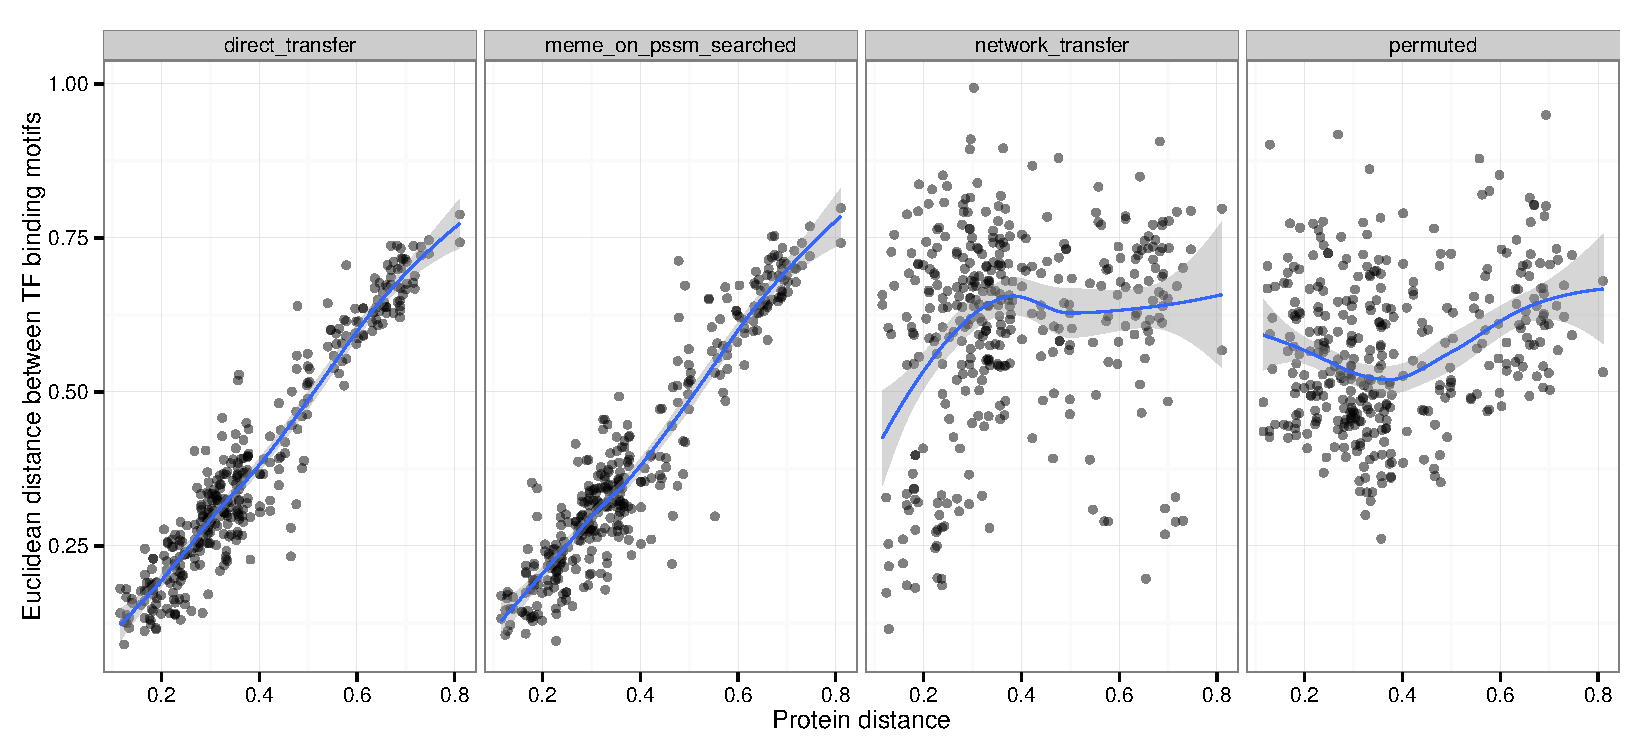
\includegraphics[width=\textwidth]{figs/plot2.pdf}
  \caption[ ]{The Euclidean distance between the true target motif and inferred
    motif.}
\label{fig:results_euclidean}
\end{figure}

\begin{figure}
  \centering
  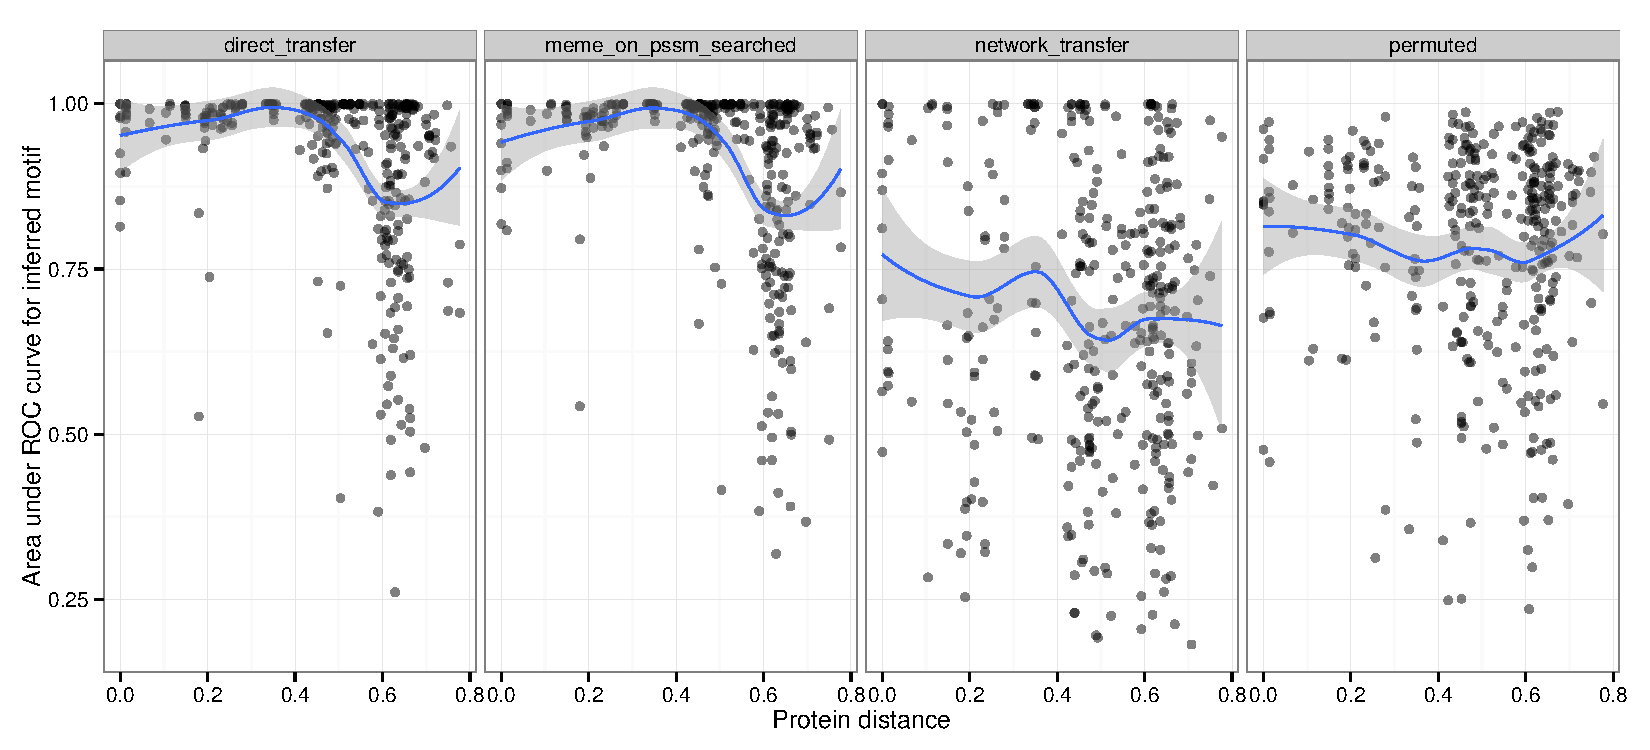
\includegraphics[width=\textwidth]{figs/plot1.pdf}
  \caption{Area under ROC curves for motifs inferred via different transfer
    methods.}
\label{fig:results_ROC}
\end{figure}

Although network transfer is often capable of inferring non-conserved motifs for
large protein distances, the permutation analysis suggests that these data
points are not statistically significant. In fact, it can be concluded that the
network transfer method does not perform well for any level of reference-target
distance overall. Our analysis demonstrating the poor performance of this method
is consistent with previous studies reporting high plasticity in transcriptional
regulatory networks and therefore weakening the assumption of functional
conservation made in network transfer~\cite{price2007orthologous,
  babu2006evolutionary, chavez2006bacterial}. In this context, our further
analysis revealed that the poor performance is due to stringent nature of the
reciprocal BLAST for ortholog detection. This results in too few promoters with
true sites for MEME to be able to detect the signal. Figure
\ref{fig:network_transfer} shows the precision ($TP/(TP+FP)$) and recall
($TP/(TP+FN)$) rates for each transferred regulon {\em before} the motif
discovery step. Here, a promoter is considered as a true positive (TP) if it
contains a true site from the target motif and selected as a target promoter to
be searched by MEME\@. False positives (FP) are promoters with no true sites but
in the collection MEME searches and false negatives (FN) are promoters with
sites but not in the collection that MEME searches for a motif. Low precision
and recall rates suggest that, in most cases, most of the operons in the
inferred regulon are not members of the true target regulon. As a result, MEME
is not able to recover the true binding motif.

\begin{figure}
  \centering
  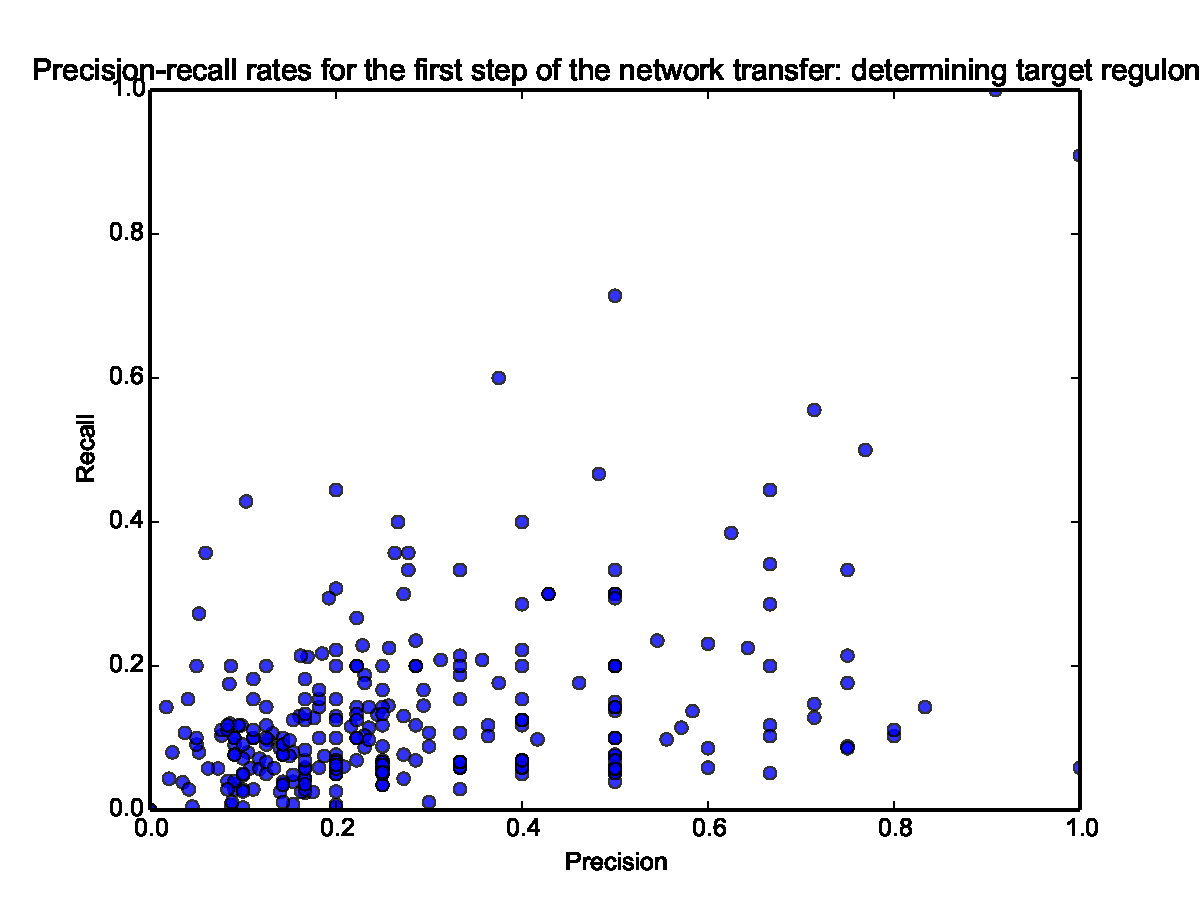
\includegraphics[width=.6\textwidth]{figs/pr.pdf}
  \caption{Precision and recall curves for the first step (i.e., regulon
    transfer) of the network transfer. }
\label{fig:network_transfer}
\end{figure}


\section{Conclusion}
In this paper, we report the first benchmarking of methods for transfer of
regulatory information across bacterial genomes. We performed experiments using
TF binding motif data compiled from CollecTF and other publicly available
databases. Our analysis suggests that the traditional approach of direct
transfer via PSSM search performs best, especially when the reference and target
species are closely related. We also tested a network transfer approach which is
based on the assumption of regulatory network conservation. In accordance with
the recent studies suggesting extensive rewiring of regulatory networks, we
found that the network transfer approach does not perform well because of small
overlap between networks and a large amount of noise in the transfer process
that overcomes the power of motif discovery method.

Our further analysis indicates that another reason for poor network transfer is
the strictness of the reciprocal BLAST-based regulon transfer method. One
direction for future work is to modify the network transfer method to use
functional similarity (e.g., clusters of orthologous groups,
COGs~\cite{tatusov1997genomic}) for regulon transfer rather than direct
orthology. With this approach, instead of considering genes that are orthologous
to those in the reference network, target genes that have same or similar
function to reference regulon are also considered for motif discovery. A second
future direction is to investigate whether combining the information from the
extended network transfer with relaxed PSSM searches can enhance the performance
of direct transfer as the similarity between reference and target motifs decays.

\bibliographystyle{unsrt}
\bibliography{/home/sefa/Dropbox/research/bib/bibliography}

\end{document}

